\documentclass[aip,pof,reprint]{revtex4-1}

\usepackage{graphicx}
\usepackage{amsmath}
\usepackage{amssymb}
\usepackage{hyperref}
\usepackage{color}

\begin{document}

\title{Convergence rate of individual and global quantities in Direct Numerical Simulations} %Title of paper

\author{C\'edric Flageul}
\email{cedric.flageul@ijs.si}
%\homepage{https://repo.ijs.si/CFLAG}
\author{Iztok Tiselj}
\email{iztok.tiselj@ijs.si}
\affiliation{Reactor engineering division,
Jo\v{z}ef Stefan institute,
Ljubljana, Slovenia}

\date{\today}

\begin{abstract}
Typical individual quantities in Direct Numerical Simulations of statistically steady flows are converging at a rate of $1/\sqrt{T}$, where $T$ is the averaging time of the simulation.
However, global quantities that represent integral momentum balance in the computational domain can exhibit a faster convergence rate of $1/T$.
This faster convergence rate is analysed and explained.
Theoretical predictions are supported with a Direct Numerical Simulation.
\end{abstract}

%\pacs{}% insert suggested PACS numbers in braces on next line

\keywords{Direct Numerical Simulation, Uncertainty Quantification, Sampling Error}

\maketitle %\maketitle must follow title, authors, abstract and \pacs

As the existing computational power available increases, Direct Numerical Simulation (DNS) establishes itself as one of the most accurate way to analyse fluid flows.
Thanks to Oliver et al. \cite{oliver}, practitioners are now able to estimate the statistical uncertainty plaguing their results.
This is a major step towards uncertainty quantification as the statistical uncertainty is usually the main source of error in DNS.

Recently, Thompson et al. \cite{thompson} proposed and applied a methodology to evaluate the statistical error plaguing the averaged velocity and the Reynolds stress in plane channel flows.
This methodology was used by Andrade et al. \cite{andrade}.
Their Figure 6 suggested a residual norm decreasing as $\frac{1}{T}$, with $T$ the averaging time.

However, following Oliver et al. \cite{oliver}, it is known that individual statistical quantities are converging slower, at a rate of $\frac{1}{\sqrt{T}}$.
This is the expected convergence rate for an uncorrelated signal, and for a weakly correlated one approaching independence at large separations, such as a turbulent signal (Theorem 27.4 in Billingsley \cite{billingsley2008probability}).

In the present paper, we show that both aforementioned convergence rates hold and are not contradictory.
This is confirmed by statistics taken from a DNS.
Thus, we demonstrate that the methodology for evaluation of statistical uncertainties proposed by Thompson et al. \cite{thompson} is not conservative as it provides an error which is converging faster than individual quantities.

The structure of the remaining part of the paper is as follows.
First, we show that the residual norms proposed by Thompson et al \cite{thompson} are converging at a rate of $\frac{1}{T}$.
Then, we show DNS results in agreement with our analysis, alongside with some concluding remarks and comments.

The following is tailored to the time scheme used by Andrade et al. \cite{andrade}.
It could be simply adapted to fit another time scheme.
The velocity in direction $i$ and at time step $n$ is written $u_i^n$.
The pressure at time step $n$ is written $p^n$.
The time step is written $dt$.
Spatial derivativation in direction $i$ is written $\partial_i$ and $\delta_{i,j}$ is the Kronecker delta.
In the present study, $X$, $Y$ and $Z$ stand for the streamwise, wall-normal and spanwise directions, respectively.
The prediction step is a combination of a $2^{nd}$ order Adams-Bashforth and Crank-Nicolson, and there is an imposed constant source term ($f$) in the streamwise direction driving the flow:
\begin{eqnarray}
\label{qdm_pred}
\frac{u_i^*-u_i^n}{dt}
& = &
- \frac{3}{2} \partial_j \left( u_i^n u_j^n \right)
+ \frac{1}{2} \partial_j \left( u_i^{n-1} u_j^{n-1} \right)
- \partial_i p^n \nonumber \\
& + & \frac{1}{Re} \partial_{jj} \left( \frac{u_i^* + u_i^n}{2} \right)
- f \delta_{iX}
\end{eqnarray}
The correction step enforces the continuity equation
\begin{equation}
\label{qdm_corr}
\frac{u_i^{n+1}-u_i^*}{dt} = - \partial_i p^{n+1} + \partial_i p^{n}
\end{equation}
as the pressure $p^{n+1}$ is obtained with the following Poisson equation:
\begin{equation}
\label{qdm_poisson}
\partial_{ii} p^{n+1} = \partial_{ii} p^{n} + \frac{\partial_i u_i^*}{dt}
\end{equation}
From equation (\ref{qdm_corr}), one can derive
\begin{equation}
\label{qdm_ustar}
u_i^* = u_i^{n+1} + dt \left( \partial_i p^{n+1} - \partial_i p^{n} \right)
\end{equation}

\begin{widetext}
Equation (\ref{qdm_ustar}) allows us to eliminate $u_i^*$.
The resulting time scheme is:
\begin{eqnarray}
\label{qdm}
\frac{u_i^{n+1}-u_i^n}{dt}
=
- \frac{3}{2} \partial_j \left( u_i^n u_j^n \right)
+ \frac{1}{2} \partial_j \left( u_i^{n-1} u_j^{n-1} \right)
- \partial_i p^{n+1} %\nonumber \\
+ \frac{1}{Re} \partial_{jj} \left( \frac{u_i^{n+1} + u_i^n}{2} + \frac{dt}{2} \partial_i \left( p^{n+1}-p^{n} \right) \right)
- f \delta_{iX}
\end{eqnarray}

At this point, the time-discrete momentum equation (\ref{qdm}) is averaged in time.
This corresponds to a summation from the time step $n=1$ to $n=N$, followed by a division by $N$:
\begin{eqnarray}
\label{qdm_sum_t}
&&
\frac{u_i^{N+1}-u_i^1}{Ndt}
+ \frac{1}{2N} \partial_j \left( u_i^{N} u_j^{N} - u_i^0 u_j^0 \right)
%\nonumber \\
- \frac{1}{NRe} \partial_{jj} \left( \frac{u_i^{N+1} - u_i^1}{2} + \frac{dt}{2} \partial_i \left( p^{N+1} - p^1 \right) \right)
+ \frac{\partial_i p^{N+1} - \partial_i p^1}{N}
\nonumber \\
& = &
\frac{ \sum_{k=1}^N
- \partial_j \left( u_i^k u_j^k \right)
- \partial_i \left( p^k \right)
+ \frac{1}{Re} \partial_{jj} \left( u_i^k \right)
- f \delta_{i,X}}{N}
\end{eqnarray}
On the right-hand side of equation (\ref{qdm_sum_t}) is the exact momentum equation averaged in time over the simulation.
Thus, the left-hand side of this equation corresponds to a residual.
When $N$ is large enough, the velocity and pressure fields at the initial time steps are independent from the ones at the final time steps.
As the flow is statistically steady, the initial and final fields are described by the same probability density function.
Therefore, the collected statistics will converge towards the exact time-averaged momentum equation at a rate of $\frac{1}{N}$, or $\frac{1}{T}$.
This convergence rate was obtained without any specific assumption.
Thus, it does not depends on the geometry or on the Reynolds number, and is valid everywhere inside the computational domain, as long as the initial turbulent flow is fully developped.

Hereafter, we focus on the streamwise and spanwise momentum equations which are useful as indicators of the statistical uncertainty in the channel flow.
Both equations are averaged over the homogeneous directions $X$ and $Z$.
Quantities averaged in space are written with one overbar.
The resulting space-averaged time-averaged discrete momentum equations are:
\begin{eqnarray}
\label{qdm_sum_x}
\frac{\overline{u_X^{N+1}}-\overline{u_X^1}}{Ndt}
+ \frac{1}{2N} \partial_Y \left( \overline{u_X^{N} u_Y^{N}} - \overline{u_X^0 u_Y^0} \right)
- \frac{1}{NRe} \partial_{YY} \left( \frac{\overline{u_X^{N+1}} - \overline{u_X^1}}{2}\right)
& = & \frac{ \sum_{k=1}^N
- \partial_Y \left( \overline{u_X^k u_Y^k} \right)
+ \frac{1}{Re} \partial_{YY} \left( \overline{u_X^k} \right)
- f}{N} \\
\label{qdm_sum_z}
\frac{\overline{u_Z^{N+1}}-\overline{u_Z^1}}{Ndt}
+ \frac{1}{2N} \partial_Y \left( \overline{u_Z^{N} u_Y^{N}} - \overline{u_Z^0 u_Y^0} \right)
- \frac{1}{NRe} \partial_{YY} \left( \frac{\overline{u_Z^{N+1}} - \overline{u_Z^1}}{2}\right)
& = & \frac{\sum_{k=1}^N
- \partial_Y \left( \overline{u_Z^k u_Y^k} \right)
+ \frac{1}{Re} \partial_{YY} \left( \overline{u_Z^k}\right)}{N}
\end{eqnarray}
\end{widetext}

To measure the convergence rate, we define the following quantities:
\begin{eqnarray}
E_0^X\left(y\right) & = & \frac{\sum_{k=1}^N -\partial_Y \left( \overline{u_X^k u_Y^k} \right)+\frac{1}{Re}\partial_{YY}\left( \overline{u_X^k} \right)-f}{N} \nonumber \\
E_0^Z\left(y\right) & = & \frac{\sum_{k=1}^N -\partial_Y \left( \overline{u_Z^k u_Y^k} \right)+\frac{1}{Re}\partial_{YY}\left( \overline{u_Z^k} \right)}{N} \nonumber \\
{\parallel{E_0^i}\parallel}^2 & = & \frac{1}{{Re}_\tau} \int_{y^+=0}^{{Re}_\tau} {E_0^i\left(y^+\right)}^2
\end{eqnarray}
Based on this, one can recover the residual error $E^i_R$, as defined by Andrade et al. \cite{andrade}:
\begin{eqnarray}
\label{definition_ER}
E^i_R \left(y^+\right) & = & \int_{l=0}^{y^+} E_0^i\left(l\right)  \\
{\parallel{E^i_R}\parallel}^2 & = & \frac{1}{{Re}_\tau} \int_{y^+=0}^{{Re}_\tau} {E^i_R \left(y^+\right)}^2
\end{eqnarray}
The residual error $E^i_U$, also defined by Andrade et al. \cite{andrade}, can be obtained by integrating $E^i_R$.
Obviously, $\parallel{E_0^i}\parallel$, $\parallel{E^i_R}\parallel$ and $\parallel {E^i_U} \parallel $ should have the same convergence rate.

For the spanwise momentum equation, the global quantity ${\parallel{E_0^Z}\parallel}^2$ is completed by the following individual quantities:
\begin{eqnarray}
Z-Conv = \frac{1}{{Re}_\tau} \int_{y^+=0}^{{Re}_\tau} \left( \frac{\sum_{k=1}^N \partial_Y \left( \overline{u_Z^k u_Y^k} \right) }{N} \right)^2 \\
Z-Diff = \frac{1}{{Re}_\tau} \int_{y^+=0}^{{Re}_\tau} \left( \frac{\sum_{k=1}^N \frac{1}{Re}\partial_{YY}\left( \overline{u_Z^k} \right) }{N} \right)^2
\end{eqnarray}

Regarding the conversion towards wall-units, a friction velocity  --- the theoretical one --- can be derived from the constant source term $f$ used in the momentum equation.
Another friction velocity --- the measured one --- can be derived from the averaged streamwise velocity.
In the present study, the former is used as it is not plagued by any statistical uncertainty.
The definition of $E^i_R$, as given by equation (\ref{definition_ER}), uses an integration constant to enforce $E^i_R \left( y^+ = 0 \right) = 0$.
In the present study, we weakly enforce this condition at $y^+=0$ by using an integration constant derived from the theoretical friction velocity, as in Andrade et al. \cite{andrade}.
This choice, combined with the symmetry of the case at hand, strongly enforces $E^i_R \left( y^+ = Re_\tau \right) = 0$.

Hereafter, we present DNS results supporting our analysis.
For convenience, all quantities plotted are integrated squared residuals.
Thus, expected convergence rates are also squared and individual quantities are expected to converge at a rate of $\frac{1}{T}$, while global ones such as ${\parallel{E_0^i}\parallel}^2$ and ${\parallel{E^i_R}\parallel}^2$ are expected to converge at a rate of $\frac{1}{T^2}$.

The present DNS was performed with the pseudo-spectral code previously used in Flageul and Tiselj \cite{flageul}.
The friction Reynolds number is $180$.
The shape and the resolution of the computation is equal to the DNS of Moser et. al. \cite{moser} $\left[ L_X = 4 \pi h, L_Y = 2h, L_Z = \frac{4 \pi h}{3}\right]$, $\Delta_X^+ = 17.7$, $0.054 \leq \Delta_Y^+ \leq 4.4$ and $\Delta_Z^+ = 5.90$.
This resolution was recognized as slightly under-resolved DNS in the study by Vreman and Kuerten \cite{vreman}.
This is not really an issue here as this paper is focused only on statistical uncertainty and not on the numerical accuracy.
The time step in the DNS is $0.027$ wall-units, and statistics are collected every $10$ time steps.
$2$ million time steps are performed, so the averaging time is $54000$ wall-units and the effective averaging time, as proposed by Vinuesa et. al. \cite{vinuesa}, is 
$T^\star = \frac{T u_\tau}{h} ~ \frac{L_X L_Z}{L_{X,min} L_{Z,min}} = 880$, with $L_{X,min} = 6h$ and $L_{Z,min} = 3h$.

\begin{figure}
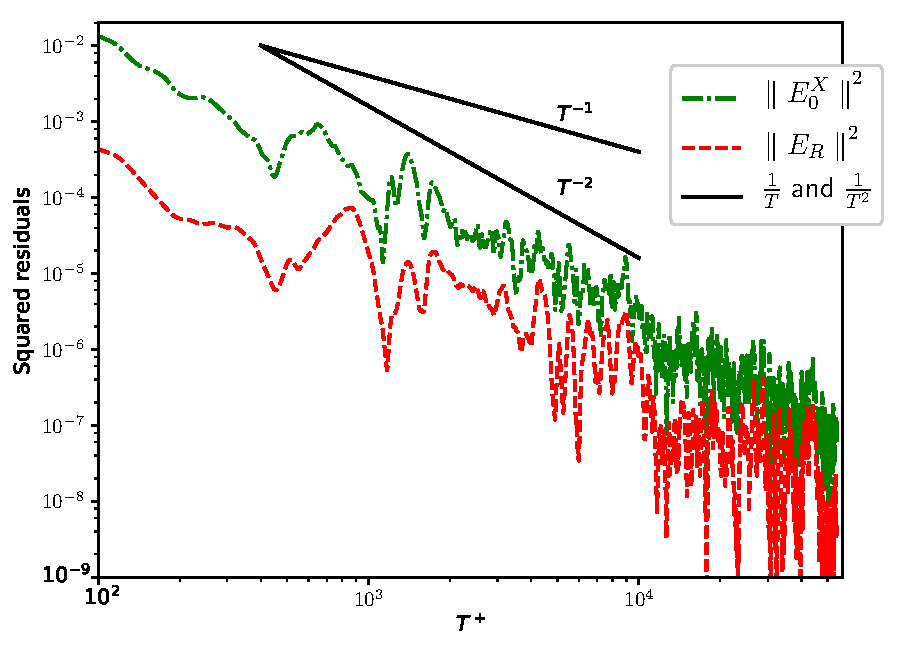
\includegraphics[width=0.5\textwidth]{streamwise_convergence.pdf}
\caption{\label{fig_x}Convergence of global quantities associated with the streamwise momentum as a function of the averaging time. Dotted green line: ${\parallel{E_0^X}\parallel}^2$. Dashed red line: ${\parallel{E^X_R}\parallel}^2$. Black lines: Convergence rates of $\frac{1}{T}$ and $\frac{1}{T^2}$.}
\end{figure}

As shown in Figure \ref{fig_x}, the global quantities ${\parallel{E_0^X}\parallel}^2$ and ${\parallel{E^X_R}\parallel}^2$ associated with the streamwise momentum equation are converging at the expected rate of $\frac{1}{T^2}$.

\begin{figure}
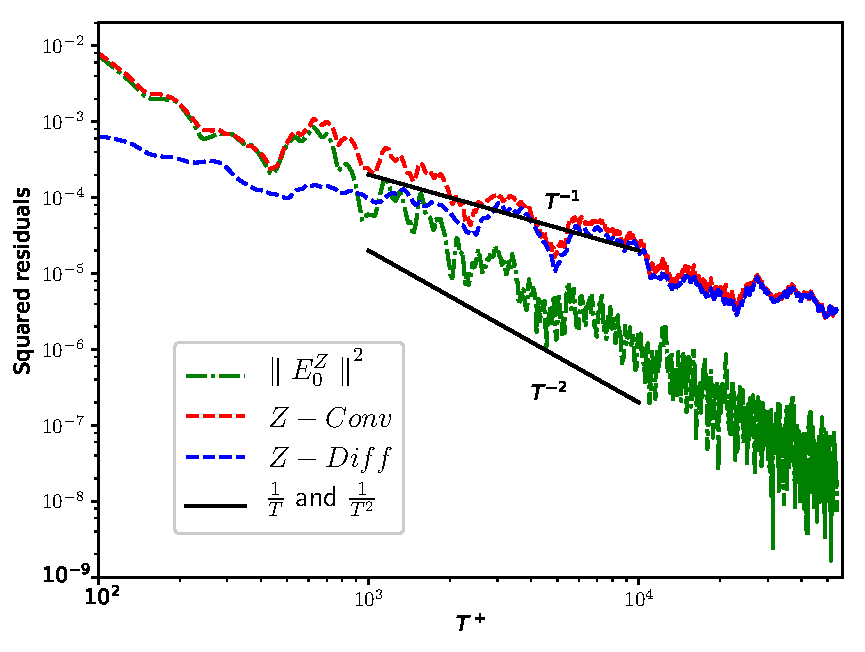
\includegraphics[width=0.5\textwidth]{spanwise_convergence.pdf}
\caption{\label{fig_z}Convergence of individual and global quantities associated with the spanwise momentum as a function of the averaging time. Dotted green line: ${\parallel{E_0^Z}\parallel}^2$. Dashed red line: $Z-Conv$. Dashed blue line: $Z-diff$. Black lines: Convergence rates of $\frac{1}{T}$ and $\frac{1}{T^2}$.}
\end{figure}

As shown in Figure \ref{fig_z}, the squared residuals associated with individual quantities are converging at a rate of $\frac{1}{T}$, while the squared residual associated with the global quantity ${\parallel{E_0^Z}\parallel}^2$ is converging at the faster rate of $\frac{1}{T^2}$.

For the sake of completeness, regressions were performed to extract the convergence rate of the quantities plotted in Figures \ref{fig_x} and \ref{fig_z}.
The regression was restricted to averaging times longer than $10^4$ time steps -- $2700$ time units -- to limit transient effects.
Table \ref{tab_conv_rate} shows that the convergence rate of global quantities is very close to the theoretical prediction.
Table \ref{tab_conv_rate_2} shows that the individual quantities are converging slightly faster than expected (Oliver et al. \cite{oliver}, Billingsley \cite{billingsley2008probability}).

\begin{table}
\caption{\label{tab_conv_rate}Convergence rate for global quantities, averaging time $T^+>2700$.}
\begin{ruledtabular}
\begin{tabular}{rcccc}
 & ${\parallel{E_0^X}\parallel}^2$ & ${\parallel{E_0^Z}\parallel}^2$ & ${\parallel{E_R^X}\parallel}^2$ & ${\parallel{E_R^Z}\parallel}^2$ \\
\hline
Convergence Rate & $T^{-2.0481}$ & $T^{-2.2370}$ & $T^{-2.0558}$ & $T^{-2.2370}$ \\
\end{tabular}
\end{ruledtabular}
\end{table}

\begin{table}
\caption{\label{tab_conv_rate_2}Convergence rate for individual quantities, averaging time $T^+>2700$.}
\begin{ruledtabular}
\begin{tabular}{rcccc}
 & $Z-Conv$ & $Z-diff$ \\
\hline
Convergence Rate & $T^{-1.0681}$ & $T^{-0.9332}$ \\
\end{tabular}
\end{ruledtabular}
\end{table}

The authors have presented an original analysis showing that different quantities can have different convergence rates, and have provided DNS evidences supporting it.
Overall, individual quantities are expected to converge at a rate of $\frac{1}{\sqrt{T}}$.
However, a few global quantities, directly related to the integral equations solved are converging faster, at a rate of $\frac{1}{T}$.
The only global quantities the authors could identify are the ones directly derived from the conservation equations solved, as expressed equation (\ref{qdm_sum_t}).

One could try to multiply equation (\ref{qdm}) by $\left( u_i^{n+1}+u_i^n \right)$ to obtain an equation for the kinetic energy as a global quantity.
However, summation over time steps no longer leads to simplification.
Thus, it seems that no other global quantity converging at a rate of $\frac{1}{T}$ can be derived on this ground, except linear transformations of the previous ones.
As integration and derivation are linear transformations, the time-averaged equation of conservation of vorticity is also a global quantity converging at a rate of $\frac{1}{T}$.

The present analysis was focused on the momentum equation, but will also apply to transported scalars, such as the temperature or the enthalpy.
In addition, this analysis is not restricted in any way to simple geometries such as the channel flow studied here and can be directly applied to DNS of more complex geometries.
The main requirement is that the case studied must be statistically steady.
The other is that the DNS should rely on a classical combination of implicit and explicit time schemes.
The presented analysis should also apply to time schemes with a variable time step.

As a side remark, our analysis shows that the residuals associated with the global momentum equation depend only on the initial and final fields.
Thus, provided one has kept those fields, one can estimate the error on the averaged momentum equation without using any averaged quantity.
Indeed, this is of very limited use, except for an efficient on-the-fly estimation of this global error during the simulation.

A potentially interesting error estimator regarding individual statistical quantities for cases with symmetry or invariance under rotation could be derived from the lack of symmetry or invariance in the measured profile.
This is left for future prospects.
As a side note, the authors would like to stress that convergence rates correspond to asymptotic limits and long averaging time can be necessary to observe them, especially for low probability events (Bauer et al. \cite{bauer2017convergence}).

The authors would like to thank the Slovenian Research Agency for funding the study under the research project P2-0026.
Data associated with the present paper are available online at \url{https://repo.ijs.si/CFLAG/convergence_rate} under the GNU GPL v3 licence.

\bibliography{FLAGEUL_TISELJ_convergence_rate}

\end{document}
